\documentclass{article}

\usepackage{graphicx}
\usepackage{wrapfig}
\usepackage{algorithmicx}
\usepackage{algpseudocode}
\usepackage{multicol}
\usepackage{multirow}
\usepackage{amsmath,amssymb,amsfonts}
\usepackage{hyperref}
\usepackage{caption}
\usepackage{subcaption}
\usepackage{float}
\usepackage{array}
\usepackage{xcolor}
\usepackage[normalem]{ulem}
% \usepackage[style=ieee]{biblatex}
\usepackage[a4paper, left=1in, right=1in, top=1in, bottom=1in]{geometry}
% \graphicspath{{pictures/}}


\begin{document}
\begin{center}
    \Large
    CSE 306 \\[10pt]
    \textbf{Computer Architecture Sessional} \\[40pt]
    
    \Large
    Assignment-2: 32-bit Floating Point Adder Simulation \\[40pt]
    
    \large
    Section - A1 \\[10pt]
    Group - 06 \\[80pt]

\end{center}
\begin{tabbing}
\large
{Members of the Group:} \\[20pt]
    i\hspace{1cm}\=2105002 - Khalid Hasan Tuhin \\[10pt]
    ii\>2105014 - K.M. Mehemud Azad \\[10pt]
    iii\>2105015 - Arnob Biswas \\[10pt]
\end{tabbing}
\newpage

\section{Introduction}
In this project, we have developed and implemented a 32-bit Floating Point Adder (FPA) circuit as a core component of our study in computer architecture. Floating Point Arithmetic (FPA) is essential in computing, as it allows for a vast range of values that can represent very small fractions as well as very large numbers, crucial for scientific calculations, engineering applications, and any task that requires precision beyond integers. A floating-point representation typically uses a standardized format to encode numbers, which includes a sign bit, an exponent, and a significand (or mantissa).
\\ \\
Our 32-bit floating point adder circuit conforms to the IEEE 754 standard, widely adopted in modern computing for floating-point arithmetic. This implementation uses a 32-bit architecture, with a single bit dedicated to the sign, nine bits to the exponent, and twenty-two bits to the significand. The sign bit indicates whether the number is positive or negative, the exponent allows for a large dynamic range by representing powers of two, and the significand encodes the precision of the number, allowing us to capture significant figures within a specified range.
\\ \\ 
This adder circuit is designed to handle the complexities of floating-point addition, including the alignment of exponents, normalization of results, and handling of edge cases like underflow, overflow, and rounding. These challenges require careful handling of binary arithmetic operations and logical circuits to ensure accuracy and efficiency, especially in cases where the exponents of the two operands differ significantly. In such cases, we implemented a mechanism to shift the significands, align them correctly, and normalize the result to maintain the IEEE 754 format.
\\ \\ 
By implementing this FPA circuit, we aimed to gain a deeper understanding of the underlying operations involved in floating-point arithmetic, which is often abstracted away in high-level programming languages. This project allowed us to explore how hardware-level operations and logic circuits work together to achieve precise and efficient calculations. The process of developing this circuit also involved learning about optimization techniques to handle common issues like rounding errors, underflows, and overflows, which are critical in ensuring that the adder performs accurately across a range of inputs.
\\ \\ 
Through this project, we have solidified our understanding of floating-point representation, binary arithmetic, and the challenges associated with precision and range in digital computing. The final implementation of our 32-bit FPA circuit provides an accurate and efficient tool for adding floating-point numbers, adhering to industry standards and preparing us for more complex digital design tasks in the field of computer architecture.

\section{Problem Specification}
This project aims to design a 32-bit floating-point adder circuit following the IEEE 754 standard. The adder will handle 1 sign bit, 9 exponent bits, and 22 significand bits, performing accurate floating-point addition with operations like exponent alignment, significand shifting, normalization, and rounding. It will also address overflow, underflow, and rounding to ensure reliable computation across diverse inputs.
\\ 

\begin{table}[h]
    \centering 
    \begin{tabular}{|c|c|c|}
        \hline 
        \textbf{Sign} & \textbf{Exponent} & \textbf{Significand} \\ 
        \hline 
        1 Bit & 9 Bit & 22 Bit \\ 
        \hline 
    \end{tabular}
    \caption{Problem Specification}
\end{table} 
\pagebreak 
\section{Flow Chart}
\begin{figure}[h]
    \centering
    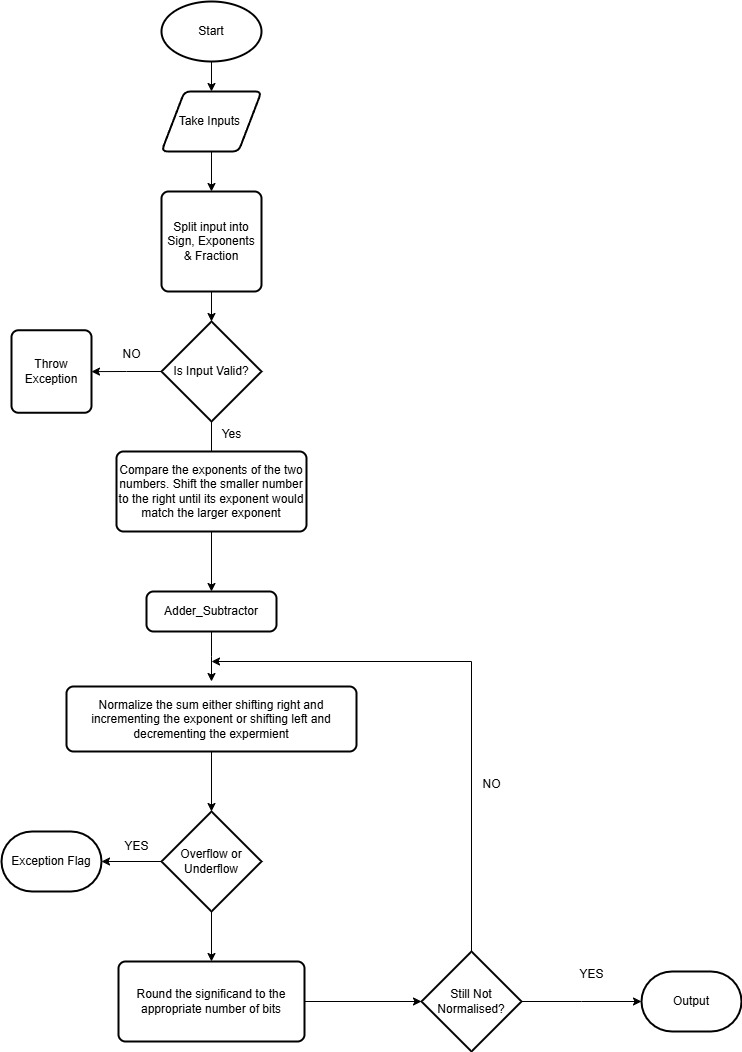
\includegraphics[width=0.7\textwidth]{flowchart.jpg}
    \caption{\textbf{Flow-Chart of the Process}}
\end{figure}
\pagebreak 
\section{High-Level Block Diagram of the Architecture}
\begin{figure}[h]
    \centering 
    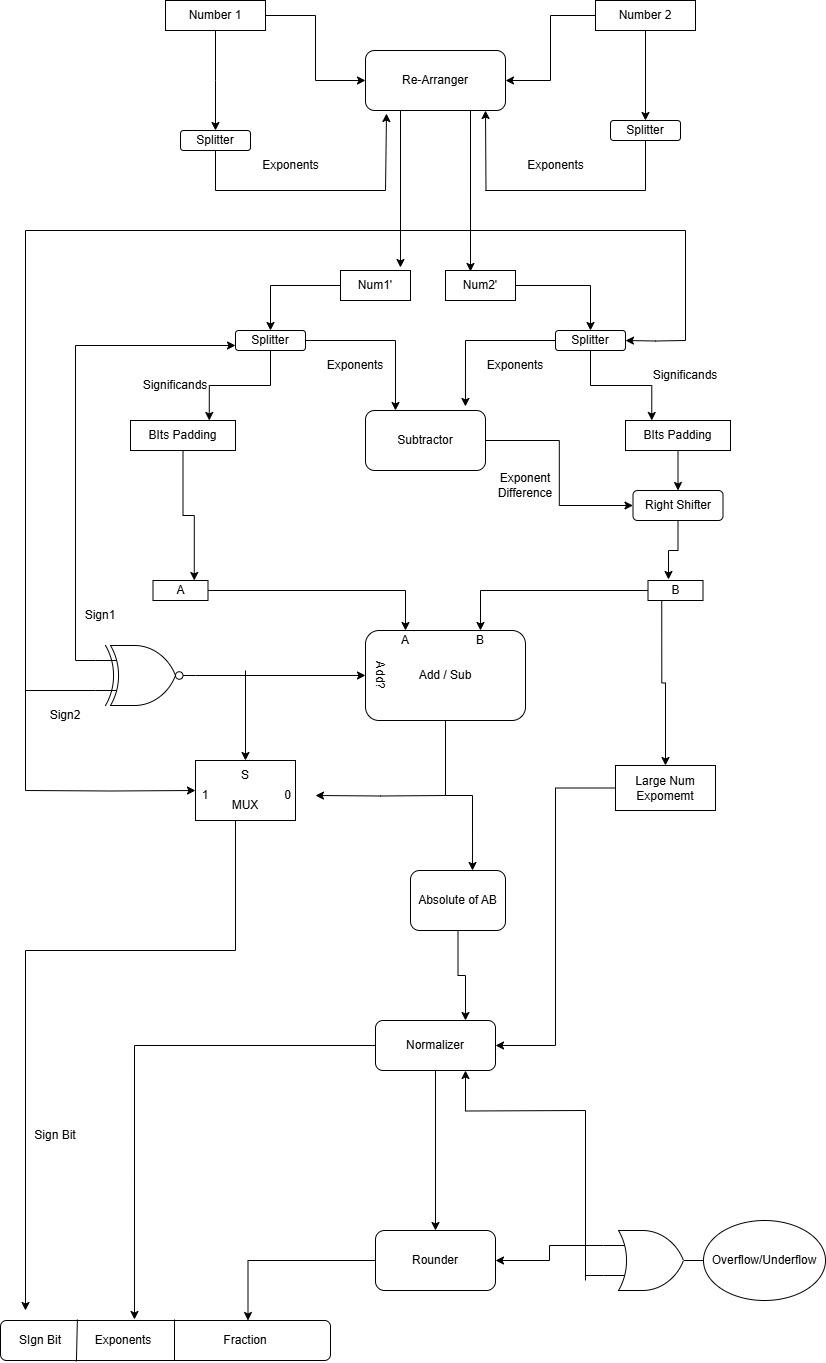
\includegraphics[width = 0.7\textwidth]{fpa.jpg}
    % \vspace{0.5cm}
    \caption{\textbf{High-Level Block Diagram of the Architectrue}}
\end{figure}
\pagebreak 

\section{Description of Modules}
Each high level module and how they work is listed below
\subsection{\textbf{Multiplexers}}
There are several multiplexer circuit each working with different input sizes.
The multiplexers that were required for this assignment are - 5×1, 8×1, 28×1,
32 × 1. They were created by chaining several 74157 MUX ICs.
\\ 
\\
\subsection{\textbf{Shifters}}
In order to shift the numbers we needed different kind of shifters for both direction. In normalization and also in exponent-equalization, the numbers needed to
be shifted by arbitrary amount. So shifters that can support arbitrary amount
shifting were required.
\\ 

Instead of making all possible shifters (1 bit shifter, 2 bit shifter, 3 bit shifter
and so on..), the design was cleverly crafted so that there are lesser number of
ICs used. Only 5 different shifters were created (1, 2, 4, 8 and 16). Each of them
having 2 inputs - the number and enable. They are designed so that when the
enable is set to 1, the number is shifted by the amount specified by the module,
otherwise the number is not changed and passed to the output. This enable
feature was achieved by introducing a MUX in the output so that when enable
is 1, the shifted number is sent to the output, otherwise the original number is
sent to the output.
\\ 

Now that the fixed amount of shifters (that can only shift by an amount that
is a whole power of 2) are ready, we can finally create arbitrary shifters. The
arbitrary right shifter (same logic for left shifter) takes 2 inputs - the number
to shift and the shift amount. Since the shift amount is specified by a binary
number, we can leverage the fact that in a binary number, each bit corresponds
to the availability of a certain power of 2. So connecting each bit to the corresponding shifter’s enable and chaining such shifters will suffice to shift by any
arbitrary amount. 

\begin{figure}[h!]
    \centering
    \begin{minipage}{0.45\textwidth}
        \centering
        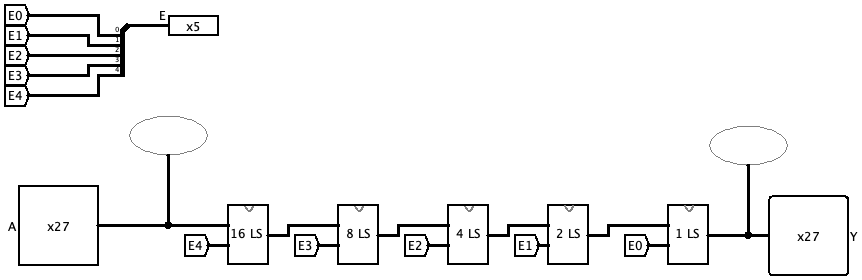
\includegraphics[width=\textwidth]{left_shifter} % Path to your first image
        \caption{Left Shifter}
        \label{fig:image1}
    \end{minipage}\hfill
    \begin{minipage}{0.45\textwidth}
        \centering
        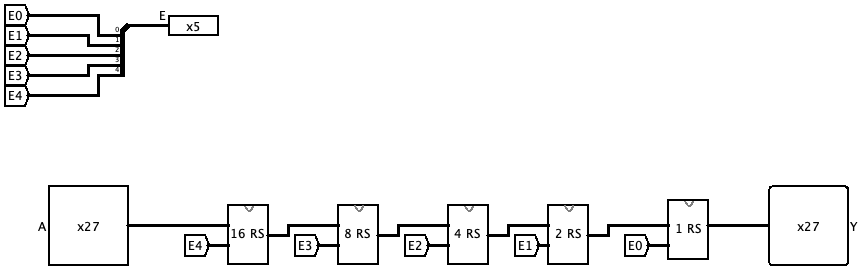
\includegraphics[width=\textwidth]{right_shifter} % Path to your second image
        \caption{Right Shifter}
        \label{fig:image2}
    \end{minipage}
\end{figure}

\subsubsection{\textbf{Shift Adapters}}
Since the exponents are 11 bits each, their difference will also be 11 bits. But
we only have 5 shifters as described in Section 5.2. So we need some sort of an
adapter that take the 11 bit difference and generate a suitable enable string for
the right shifter. This adapter basically compares the highest possible enable
value (for example it does not make sense to shift a 32 bit number more than
32 bit to the right) and the exponent difference. If the exponent difference is
larger than expected than it sets all the shifters’ enable to high, thus enabling all shifters. Otherwise it reads the last 5 bits of the exponent difference and
sends them as the enable string.
\pagebreak 
\begin{figure}[h]
    \centering
    \begin{minipage}{0.45\textwidth}
        \centering
        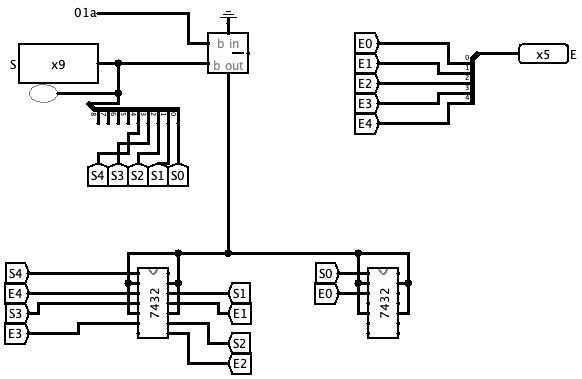
\includegraphics[width=\textwidth]{adapter} % Path to your first image
        \caption{Adapter}
        \label{fig:image1}
    \end{minipage}\hfill
    \begin{minipage}{0.45\textwidth}
        \centering
        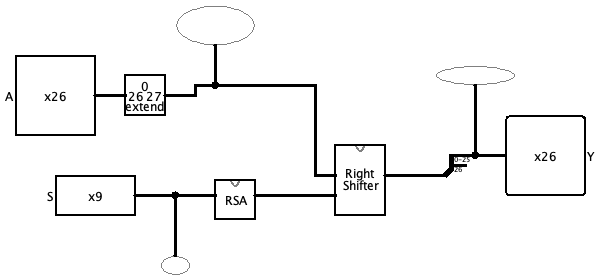
\includegraphics[width=\textwidth]{wrapper} % Path to your second image
        \caption{Wrapper}
        \label{fig:image2}
    \end{minipage}
\end{figure}

\subsection{\textbf{Re-Arranger}}
The exponents of the numbers need to be equal in order for the significands to
be passed to the adder. To do that, we first need to find the difference of their
exponent and shift the smaller exponent number to the right. So we clearly
need a distinction based on the exponent. The Re-arranger module takes 2
numbers as the base number(A, B) and 2 other decider numbers(P, Q) and
re-arrange the number based on the decider numbers. It outputs 2 numbers -
smaller and larger. If P > Q then smaller = A and larger = B. The alternative
case happens when P < Q.
\\ 

This is achieved by using a subtractor circuit as a comparator and comparing
the deciders. Then the comparison result is fed into 2 multiplexers that finally
re-arrange the base numbers and output smaller and larger. 

\begin{figure}[h]
    \centering 
    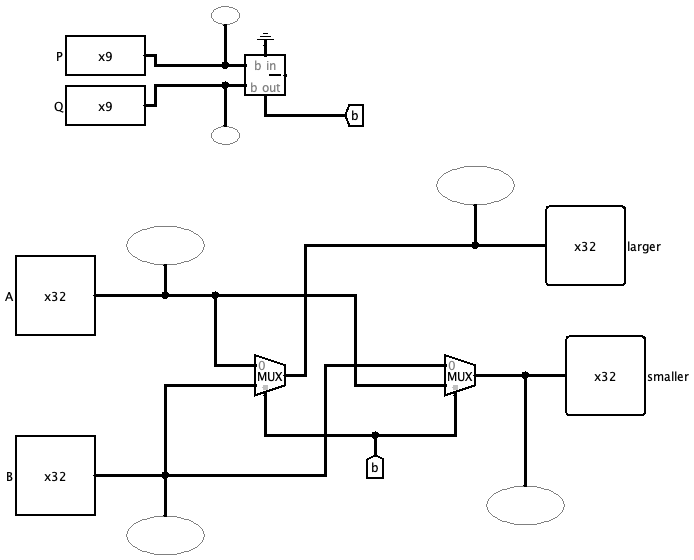
\includegraphics[width = 0.7\textwidth]{rearranger}
    % \vspace{0.5cm}
    \caption{Re-arranger}
\end{figure}

\subsection{\textbf{Priority Encoder}}
We need to use a 32-bit priority encoder for normalization (explained further
in Section - 5.5). However, 8 × 3 or 10 × 4 priority encoders are the only ones
available. Therefore, we first cascade two 74148 (8 × 3) priority encoders to
create a 16 × 4 priority encoder before creating our 32-bit priority encoder. A
second 16 × 4 priority encoder is made in a similar manner. Now we cascade
our 16×4 priority encoders to create 32×5 priority encoder. Therefore, we can
use four 74148 (8 × 3 Priority encoder) ICs to create a 32 × 5 priority encoder.
\\ 
\\ 
\subsubsection{\textbf{Cascading two 8 × 3 priority encoders}}
74148 has 8 input pins, 3 output pins, 1 enable input (EI), 1 enable output (EO)
and 1 group signal (GS) pin. We have two ICs of 74148 (IC1 and IC2). Input
8 to input 15 is connected to IC1 and input 0 to input 7 is connected to IC2.
EI of IC2 is connected to the EO of IC1. Output 3 is obtained from IC1’s GS.
Output-2 is taken from O2 (IC1) AND O1(IC2). In a similar manner, output-1
and output-0 are also obtained by applying the AND operation to IC1 and IC2’s
outputs. Another 16 × 4 priority encoder is created using two 74148 ICs (IC3
and IC4).
\begin{figure}[h]
    \centering 
    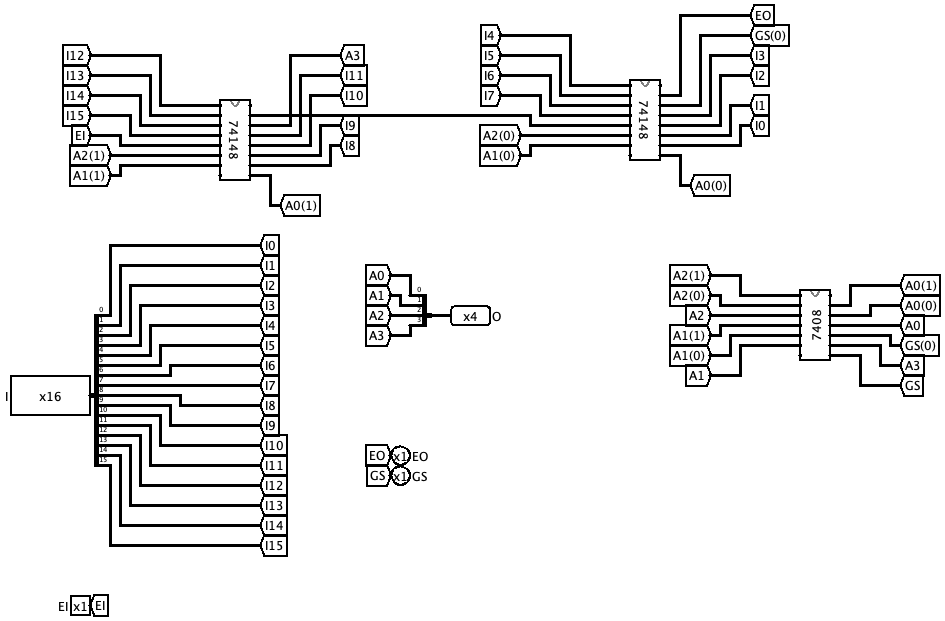
\includegraphics[width = 0.7\textwidth]{16_4}
    % \vspace{0.5cm}
    \caption{Cascading two 8x3 priority encoders}
\end{figure}
\subsubsection{\textbf{Cascading two 16 × 4 priority encoders}}
It’s the same procedure as before. Instead of using the 74148 IC as our base
component, we use the 16 × 4 encoder (described in Section 5.4.1) and cascade
2 of them to achieve a 32 × 5 encoder.
\begin{figure}[h]
    \centering 
    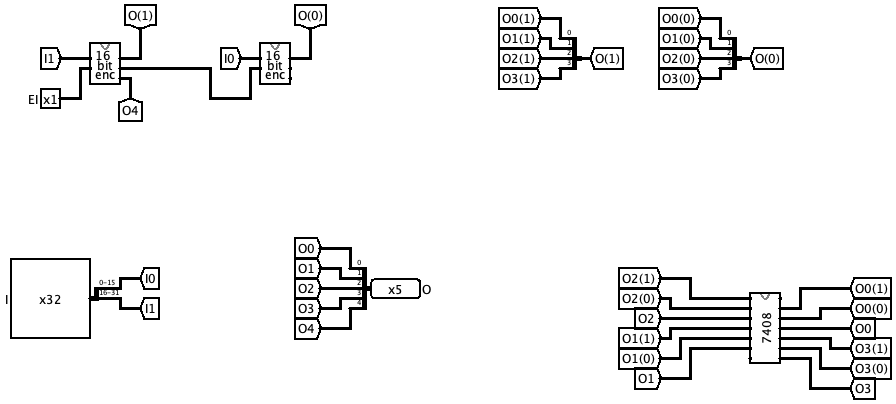
\includegraphics[width = 0.7\textwidth]{32_5}
    % \vspace{0.5cm}
    \caption{Cascading two 16x4 priority encoders}
\end{figure}
\pagebreak
\subsubsection{\textbf{32-bit input high encoder}}
This is a wrapper around the 32 bit encoder described in Section 5.4.2. To enable
active high input, we first invert the input. Our module has an additional pin
that we refer to as 1 based indexing. The output is incremented when this pin
is set high.
\begin{figure}[h]
    \centering 
    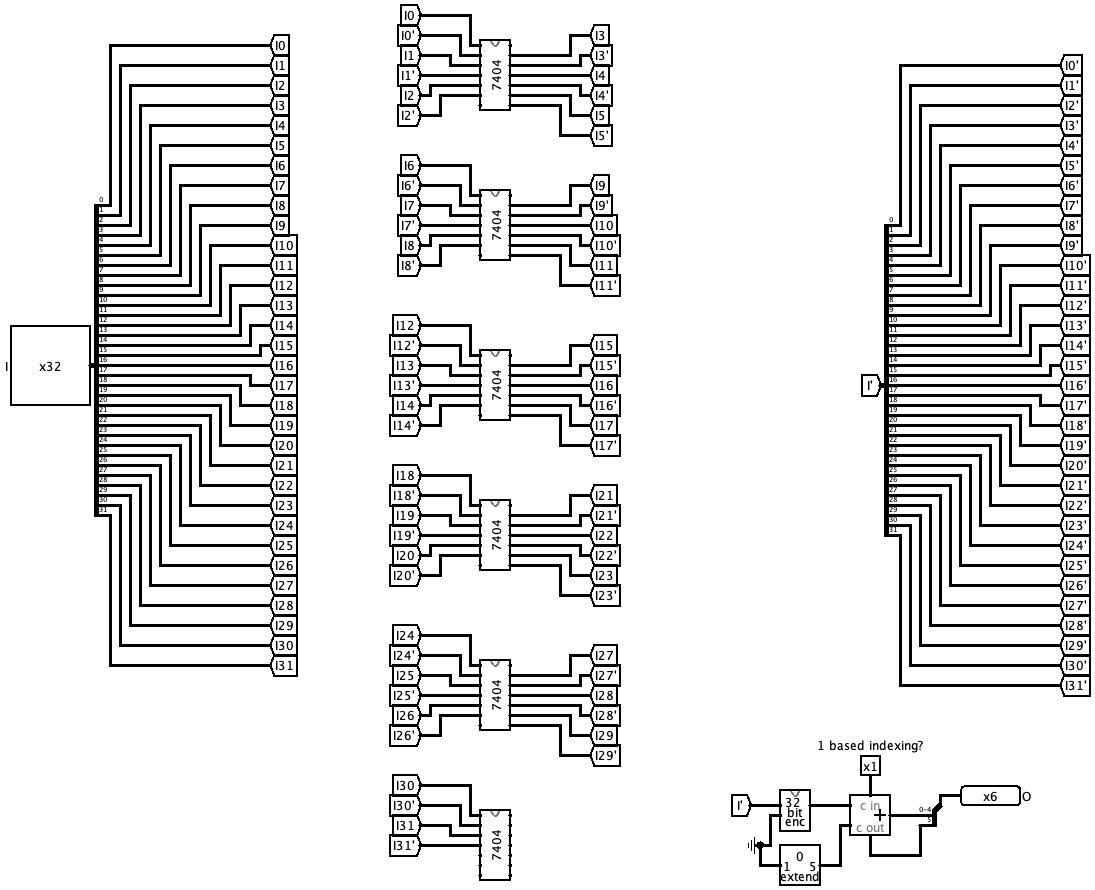
\includegraphics[width = 0.7\textwidth]{32high}
    % \vspace{0.5cm}
    \caption{32-bit input high encoder}
\end{figure}
\subsection{\textbf{Normalization}}
After addition the sum could become denormalized. In that case we have to
normalize the result. Let's say the sum looks like this: $d_1d_0.d_{-1}d_{-2}...d_{-20}.$
Then the normalization process can be described in 3 cases -
\\ 
$d_1d_0 = 01 $ The number is already normalized \\ 
$d_1d_0 = 1$x  Shift the number 1 bit to the right (hence increment the exponent) \\
$d_1d_0 = 00 $ The number needs to be left shifted to bring a 1 after the radix
point to the front of the number.
\\

The last case is a little different than the other cases since it requires finding
the first 1 after the radix point when scanned from left to right. If the first 1
is found at position $d_n$ than the number has to be shifted n bits to the left.
Note that in this example, $d_i = 0; \forall{i} < n$. The bits to the right of the first 1
do not matter. So it is clear that the first 1 has more priority than the other 1s
that follow. And we also want the position of the first 1 in binary so that this
can be directly fed into the enables of the shifters as described in Section 5.2.
This process can be done by using a priority encoder.
\\ 

But the basic 32 bit priority encoder (Section 5.4.2) has active low input and
active low output. But the bits of our significand are active high. So instead,
we use the 32-bit input high encoder (Section 5.4.3). However, there’s no need
to invert the outputs. For normalization, lets say we have 1 in the 20th bit. So,
the number needs to be shifted by 1 bit to the left. Consequently, our priority
encoder should give us 00001. We send our 20th bit to our priority encoder’s
input-31. The output we get is 00000 but our required output is 00001. That
can be achieved by setting the 1 based indexing pin high.
\\ 

After shifting the significand to the left, the exponent must also be reduced
by the shift amount.

The normalizer is the main module that handles the overflow and underflow.
Basically, after left shifting, if all of the bits of the exponent are 1, or there is
a carry generated while incrementing the exponent, this is considered to be an
overflow. As neither fall on the domain of floating point number (Note that an
exponent having all bits set is reserved).
\\ 

And after left shifting, if a borrow is generated while subtracting from the
exponent, an underflow occurs and gets reported.

\begin{figure}[h]
    \centering 
    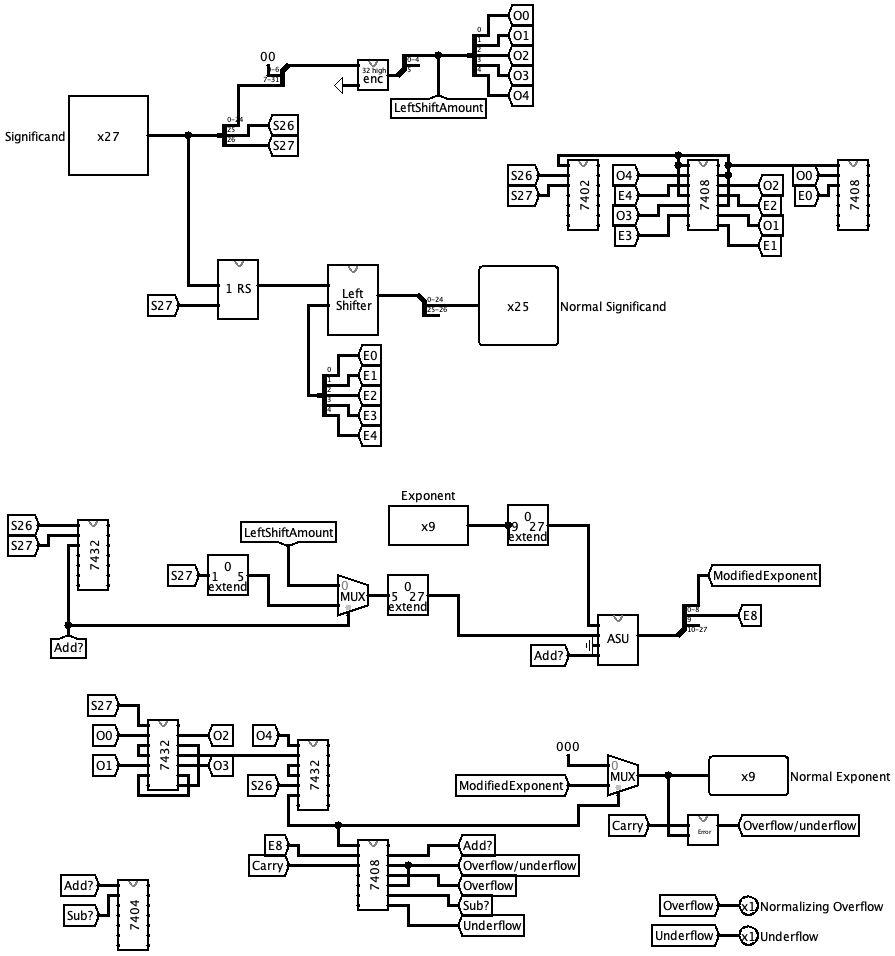
\includegraphics[width = 0.7\textwidth]{normalizer}
    % \vspace{0.5cm}
    \caption{Normalizer}
\end{figure}
\pagebreak 
\subsection{\textbf{Rounder}}
The rounder is responsible for rounding the result and storing only the limited
number of bits (in this assignment, 20 bits) in the significand segment of the
result.
\\
Initially before exponent equalization, three 0 bits are added to the right of the
number. But after the whole addition process, we can not store those bits as
our memory is limited. But those bits help us store the closest result by approximating it. The 3 bits are called the guard bit, the round bit and the sticky
bit (G, R, S).
\\

By the IEEE 754 standard, the approximation is achieved in the following
manner-
\\ 

From this table this is apparent that we only add 1 when the guard bit (G)
is 1 AND either of the round bit (R) OR the sticky bit (S) OR the last bit of
the significand is 1. So we add 1 when G(R + S + d0) = 1. In other words, we
add G(R + S + d0) to our 20 bit significand.
\\ 

The number can become denormalized after rounding up or rounding to
even. In that case we have to shift the number 1 bit to the right and hence
increment the exponent. Because the exponent is being incremented, there can
be scenarios where the exponent is too large, thus an overflow. So the rounder
also reports such overflows.
\begin{table}[h!]
    \centering
    \begin{tabular}{|c|c|c|c|c|}
        \hline
        \textbf{G} & \textbf{R} & \textbf{S} & \textbf{Process} & \textbf{Comment} \\
        \hline
        0 & 0 & 0 & Truncate       & Add 0 to the actual significand \\
        \hline
        0 & 0 & 1 & Truncate       & Add 0 to the actual significand \\
        \hline
        0 & 1 & 0 & Truncate       & Add 0 to the actual significand \\
        \hline
        0 & 1 & 1 & Truncate       & Add 0 to the actual significand \\
        \hline
        1 & 0 & 0 & Round to even  & Add 1 if the last bit of actual significand is 1 \\
        \hline
        1 & 0 & 1 & Round up       & Add 1 to the actual significand \\
        \hline
        1 & 1 & 0 & Round up       & Add 1 to the actual significand \\
        \hline
        1 & 1 & 1 & Round up       & Add 1 to the actual significand \\
        \hline
    \end{tabular}
    \caption{Rounder Truth Table}
    \label{table:rounder-truth-table}
\end{table}

\begin{figure}[h]
    \centering 
    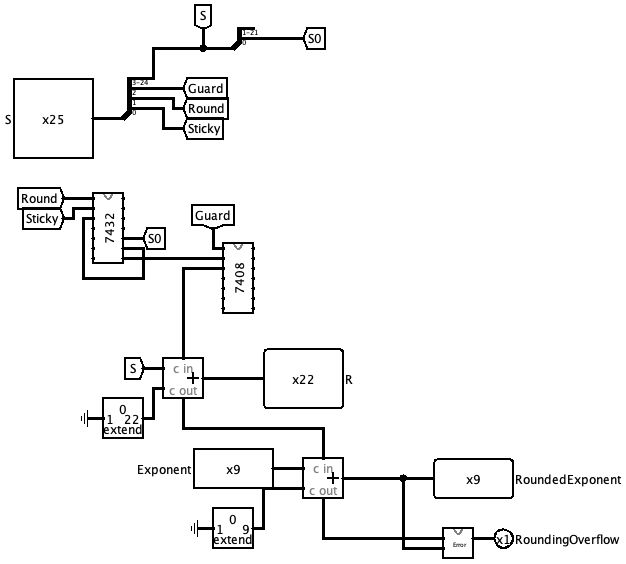
\includegraphics[width = 0.7\textwidth]{rounder}
    % \vspace{0.5cm}
    \caption{Rounder}
\end{figure}
\pagebreak 
\section{Complete Circuit Diagram} 
\begin{figure}[h]
    \vspace{4cm}
    \centering
    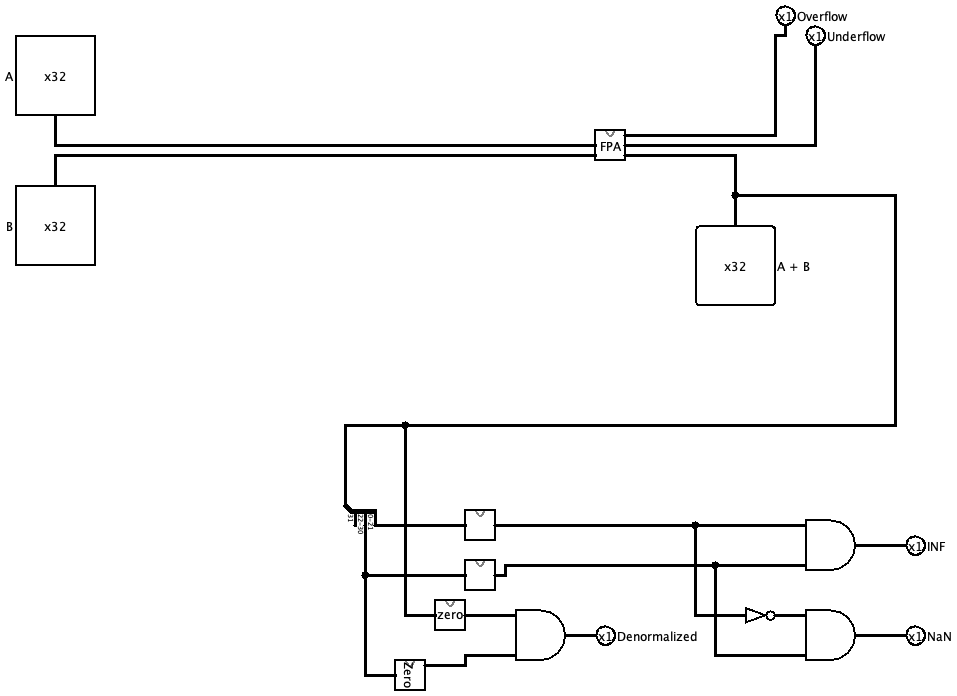
\includegraphics[width = 0.8\textwidth]{full_circuit}
    \caption{\textbf{Complete Circuit Diagram}}
\end{figure}
\pagebreak
\section{ ICs Used with Count as a Chart}

\begin{table}[h!]
    \centering
    \begin{tabular}{|c|c|}
    \hline
    \textbf{Component} & \textbf{Count} \\
    \hline
    7486 & 1 \\
    \hline
    7402 & 1 \\
    \hline
    7404 & $ 3$ \\
    \hline
    7432 & $ 23$ \\
    \hline
    7408 & $ 4$ \\
    \hline
    74157 & $ 2$ \\
    \hline
    Sub & $ 4$ \\
    \hline
    Add & $ 3$ \\
    \hline
    Mux & $ 15$ \\
    \hline
    Priority Encoder & 1 \\
    \hline
    \textbf{Total IC Count} & \textbf{57} \\
    \hline
    \textbf{Gate Counts} & \textbf{10 (left shifter + right shifter)} \\
    \hline
    \end{tabular}
    \caption{Component Counts}
    \end{table}
\section{ Simulator Software with Version}
Logisim 2.7.1 has been used for this assignment.
\\ 
\\ 
\section{Discussion}
To solve the problem, we initially focused on thoroughly understanding the theory of floating-point arithmetic (FPA). However, we soon realized that relying solely on theoretical knowledge from books left us unprepared for certain implementation details, which had to be addressed manually during the actual circuit design. This process presented several challenges along the way.
Challenges Faced - 
\\ 

\begin{itemize}
    \item \textbf{Miscalculations in Bit-Length : }
    While constructing the FPA, we needed to build right shifters, left shifters, and adder/subtractor units of specific bits. Unfortunately, we miscalculated and built them with 27 bits instead of the required 26 bits. This misstep stemmed from the complexity of the FPA workflow. From a high-level perspective, such intricacies can make it easy to overlook or miscalculate 1 or 2 extra bits—a recurring issue during the project.
    Overflow and Underflow Handling
    \item \textbf{Overflow and Underflow Handling : }
    Implementing overflow and underflow mechanisms proved to be one of the most challenging aspects. We had to not only grasp the theoretical concepts but also consider potential corner cases that might arise. For example, our initial implementation of the rounding mechanism lacked an exponent overflow check, which led to issues that had to be resolved later.
    \item \textbf{Normalizer Complexity : }
    Designing the normalizer was another intricate and time-consuming task. It required integrating shifters and accounting for several cases. Specifically, we had to determine whether to add or subtract based on the values of the 26th and 25th bits, while also addressing overflow and underflow scenarios during normalization.
    \item \textbf{Handling Special Cases (e.g., Zeros) : }
    Addressing corner cases required additional checks, especially for handling operations involving zeros. Initially, our circuit correctly handled cases like 5.2 + 0 but failed with 0 + 5.2. We also implemented a rearranger-shift adapter circuit, which ensured the shifter only shifted up to 32 bits even when the difference between the exponents exceeded 26.
    \item \textbf{Approach and Design : }
    To create a functional and efficient design, we combined built-in circuits from the Logisim library with our custom circuits. This hybrid approach allowed us to maintain a minimalist yet fully functional design.
    \item \textbf{Conclusion : }
    Designing and implementing the floating-point adder was an engaging and enlightening experience. It deepened our understanding of the inner workings of FPAs and highlighted the challenges of translating theoretical knowledge into practical implementation. Despite the obstacles, this project was a rewarding exercise in circuit design and problem-solving.
\end{itemize}
 
\section{Contribution of Each Member} 
\textbf{2105002 - Khalid Hasan Tuhin} 
\begin{itemize}
    \item Developped the Denormalizer, INF and Nan logic 
    \item Developped the zero checkers, one checkers and Re-arranger circuit 
    \item Report(section-1, section-2, section-5)
\end{itemize} 
\textbf{2105014 - K.M. Mehemud Azad}
\begin{itemize}
    \item Developped the Rounder, Normalizer circuit 
    \item Developped the Mux 
    \item Report(section-7,section-8,section-9)
\end{itemize} 
\textbf{2105015 - Arnob Biswas} 
\begin{itemize}
    \item Developped the flowchart, block diagram of the process and overflow/underflow
    \item Designed the adder and assembled components 
    \item Report(section-3, section-4,section-6)
\end{itemize}
\end{document}
